\documentclass{standalone}
\usepackage{tikz}
\usetikzlibrary{patterns, positioning}

\begin{document}
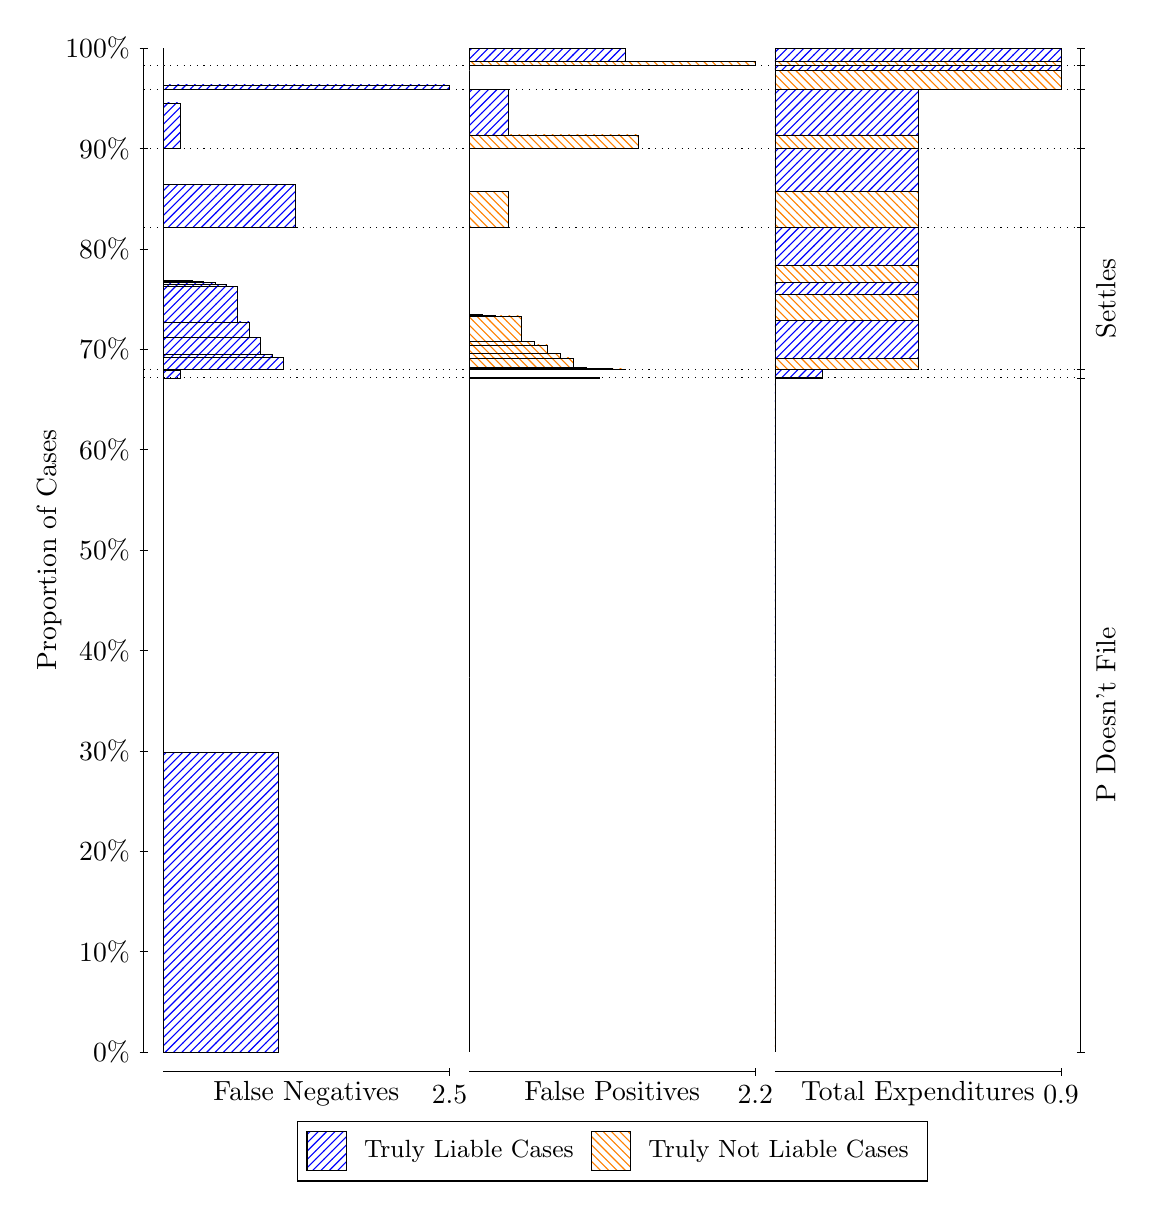
\begin{tikzpicture}
\draw[black, very thin] (1.5,1.75) -- (1.5,14.5);
\node[rotate=90, anchor=center] at (0.3, 8.125) {Proportion of Cases};
\draw[black, very thin] (1.45,1.75) -- (1.55,1.75);
\node[anchor=east] at (1.45, 1.75) {0\%};
\draw[black, very thin] (1.45,3.025) -- (1.55,3.025);
\node[anchor=east] at (1.45, 3.025) {10\%};
\draw[black, very thin] (1.45,4.3) -- (1.55,4.3);
\node[anchor=east] at (1.45, 4.3) {20\%};
\draw[black, very thin] (1.45,5.575) -- (1.55,5.575);
\node[anchor=east] at (1.45, 5.575) {30\%};
\draw[black, very thin] (1.45,6.85) -- (1.55,6.85);
\node[anchor=east] at (1.45, 6.85) {40\%};
\draw[black, very thin] (1.45,8.125) -- (1.55,8.125);
\node[anchor=east] at (1.45, 8.125) {50\%};
\draw[black, very thin] (1.45,9.4) -- (1.55,9.4);
\node[anchor=east] at (1.45, 9.4) {60\%};
\draw[black, very thin] (1.45,10.675) -- (1.55,10.675);
\node[anchor=east] at (1.45, 10.675) {70\%};
\draw[black, very thin] (1.45,11.95) -- (1.55,11.95);
\node[anchor=east] at (1.45, 11.95) {80\%};
\draw[black, very thin] (1.45,13.225) -- (1.55,13.225);
\node[anchor=east] at (1.45, 13.225) {90\%};
\draw[black, very thin] (1.45,14.5) -- (1.55,14.5);
\node[anchor=east] at (1.45, 14.5) {100\%};

\draw[black, very thin] (13.4,1.75) -- (13.4,14.5);
\draw[black, very thin] (13.35,1.75) -- (13.45,1.75);
\node[anchor=west] at (13.35, 1.75) {};
\draw[black, very thin] (13.35,10.311) -- (13.45,10.311);
\node[anchor=west] at (13.35, 10.311) {};
\draw[black, very thin] (13.35,10.422) -- (13.45,10.422);
\node[anchor=west] at (13.35, 10.422) {};
\draw[black, very thin] (13.35,12.224) -- (13.45,12.224);
\node[anchor=west] at (13.35, 12.224) {};
\draw[black, very thin] (13.35,13.228) -- (13.45,13.228);
\node[anchor=west] at (13.35, 13.228) {};
\draw[black, very thin] (13.35,13.972) -- (13.45,13.972);
\node[anchor=west] at (13.35, 13.972) {};
\draw[black, very thin] (13.35,14.276) -- (13.45,14.276);
\node[anchor=west] at (13.35, 14.276) {};
\draw[black, very thin] (13.35,14.5) -- (13.45,14.5);
\node[anchor=west] at (13.35, 14.5) {};

\draw[black, very thin, pattern color=blue, pattern=north east lines] (1.75,1.75) rectangle (3.2033,5.5553);
\draw[black, very thin, pattern color=orange, pattern=north west lines] (1.75,5.5553) rectangle (1.75,10.311);
\draw[black, very thin, pattern color=blue, pattern=north east lines] (1.75,10.311) rectangle (1.968,10.411);
\draw[black, very thin, pattern color=orange, pattern=north west lines] (1.75,10.411) rectangle (1.75,10.422);
\draw[black, very thin, pattern color=blue, pattern=north east lines] (1.75,10.422) rectangle (3.276,10.573);
\draw[black, very thin, pattern color=blue, pattern=north east lines] (1.75,10.573) rectangle (3.1307,10.613);
\draw[black, very thin, pattern color=blue, pattern=north east lines] (1.75,10.613) rectangle (2.9853,10.828);
\draw[black, very thin, pattern color=blue, pattern=north east lines] (1.75,10.828) rectangle (2.84,11.021);
\draw[black, very thin, pattern color=blue, pattern=north east lines] (1.75,11.021) rectangle (2.6947,11.47);
\draw[black, very thin, pattern color=blue, pattern=north east lines] (1.75,11.47) rectangle (2.5493,11.498);
\draw[black, very thin, pattern color=blue, pattern=north east lines] (1.75,11.498) rectangle (2.404,11.528);
\draw[black, very thin, pattern color=blue, pattern=north east lines] (1.75,11.528) rectangle (2.2587,11.538);
\draw[black, very thin, pattern color=blue, pattern=north east lines] (1.75,11.538) rectangle (2.1133,11.549);
\draw[black, very thin, pattern color=orange, pattern=north west lines] (1.75,11.549) rectangle (1.75,12.224);
\draw[black, very thin, pattern color=blue, pattern=north east lines] (1.75,12.224) rectangle (3.4213,12.768);
\draw[black, very thin, pattern color=orange, pattern=north west lines] (1.75,12.768) rectangle (1.75,13.228);
\draw[black, very thin, pattern color=blue, pattern=north east lines] (1.75,13.228) rectangle (1.968,13.802);
\draw[black, very thin, pattern color=orange, pattern=north west lines] (1.75,13.802) rectangle (1.75,13.972);
\draw[black, very thin, pattern color=blue, pattern=north east lines] (1.75,13.972) rectangle (5.3833,14.031);
\draw[black, very thin, pattern color=orange, pattern=north west lines] (1.75,14.031) rectangle (1.75,14.276);
\draw[black, very thin, pattern color=orange, pattern=north west lines] (1.75,14.276) rectangle (1.75,14.335);
\draw[black, very thin, pattern color=blue, pattern=north east lines] (1.75,14.335) rectangle (1.75,14.5);
\draw[black, very thin, pattern color=orange, pattern=north west lines] (5.6333,1.75) rectangle (5.6333,6.5059);
\draw[black, very thin, pattern color=blue, pattern=north east lines] (5.6333,6.5059) rectangle (5.6333,10.311);
\draw[black, very thin, pattern color=orange, pattern=north west lines] (5.6333,10.311) rectangle (7.2848,10.322);
\draw[black, very thin, pattern color=blue, pattern=north east lines] (5.6333,10.322) rectangle (5.6333,10.422);
\draw[black, very thin, pattern color=orange, pattern=north west lines] (5.6333,10.422) rectangle (7.6152,10.425);
\draw[black, very thin, pattern color=orange, pattern=north west lines] (5.6333,10.425) rectangle (7.45,10.427);
\draw[black, very thin, pattern color=orange, pattern=north west lines] (5.6333,10.427) rectangle (7.2848,10.435);
\draw[black, very thin, pattern color=orange, pattern=north west lines] (5.6333,10.435) rectangle (7.1197,10.442);
\draw[black, very thin, pattern color=orange, pattern=north west lines] (5.6333,10.442) rectangle (6.9545,10.566);
\draw[black, very thin, pattern color=orange, pattern=north west lines] (5.6333,10.566) rectangle (6.7894,10.625);
\draw[black, very thin, pattern color=orange, pattern=north west lines] (5.6333,10.625) rectangle (6.6242,10.73);
\draw[black, very thin, pattern color=orange, pattern=north west lines] (5.6333,10.73) rectangle (6.4591,10.772);
\draw[black, very thin, pattern color=orange, pattern=north west lines] (5.6333,10.772) rectangle (6.2939,11.097);
\draw[black, very thin, pattern color=blue, pattern=north east lines] (5.6333,11.097) rectangle (5.9636,11.108);
\draw[black, very thin, pattern color=blue, pattern=north east lines] (5.6333,11.108) rectangle (5.7985,11.118);
\draw[black, very thin, pattern color=blue, pattern=north east lines] (5.6333,11.118) rectangle (5.6333,12.224);
\draw[black, very thin, pattern color=orange, pattern=north west lines] (5.6333,12.224) rectangle (6.1288,12.684);
\draw[black, very thin, pattern color=blue, pattern=north east lines] (5.6333,12.684) rectangle (5.6333,13.228);
\draw[black, very thin, pattern color=orange, pattern=north west lines] (5.6333,13.228) rectangle (7.7803,13.398);
\draw[black, very thin, pattern color=blue, pattern=north east lines] (5.6333,13.398) rectangle (6.1288,13.972);
\draw[black, very thin, pattern color=orange, pattern=north west lines] (5.6333,13.972) rectangle (5.6333,14.216);
\draw[black, very thin, pattern color=blue, pattern=north east lines] (5.6333,14.216) rectangle (5.6333,14.276);
\draw[black, very thin, pattern color=orange, pattern=north west lines] (5.6333,14.276) rectangle (9.2667,14.335);
\draw[black, very thin, pattern color=blue, pattern=north east lines] (5.6333,14.335) rectangle (7.6152,14.5);
\draw[black, very thin, pattern color=orange, pattern=north west lines] (9.5167,1.75) rectangle (9.5167,6.5059);
\draw[black, very thin, pattern color=blue, pattern=north east lines] (9.5167,6.5059) rectangle (9.5167,10.311);
\draw[black, very thin, pattern color=orange, pattern=north west lines] (9.5167,10.311) rectangle (10.122,10.322);
\draw[black, very thin, pattern color=blue, pattern=north east lines] (9.5167,10.322) rectangle (10.122,10.422);
\draw[black, very thin, pattern color=orange, pattern=north west lines] (9.5167,10.422) rectangle (11.333,10.556);
\draw[black, very thin, pattern color=blue, pattern=north east lines] (9.5167,10.556) rectangle (11.333,11.044);
\draw[black, very thin, pattern color=orange, pattern=north west lines] (9.5167,11.044) rectangle (11.333,11.369);
\draw[black, very thin, pattern color=blue, pattern=north east lines] (9.5167,11.369) rectangle (11.333,11.52);
\draw[black, very thin, pattern color=orange, pattern=north west lines] (9.5167,11.52) rectangle (11.333,11.736);
\draw[black, very thin, pattern color=blue, pattern=north east lines] (9.5167,11.736) rectangle (11.333,12.224);
\draw[black, very thin, pattern color=orange, pattern=north west lines] (9.5167,12.224) rectangle (11.333,12.684);
\draw[black, very thin, pattern color=blue, pattern=north east lines] (9.5167,12.684) rectangle (11.333,13.228);
\draw[black, very thin, pattern color=orange, pattern=north west lines] (9.5167,13.228) rectangle (11.333,13.398);
\draw[black, very thin, pattern color=blue, pattern=north east lines] (9.5167,13.398) rectangle (11.333,13.972);
\draw[black, very thin, pattern color=orange, pattern=north west lines] (9.5167,13.972) rectangle (13.15,14.216);
\draw[black, very thin, pattern color=blue, pattern=north east lines] (9.5167,14.216) rectangle (13.15,14.276);
\draw[black, very thin, pattern color=orange, pattern=north west lines] (9.5167,14.276) rectangle (13.15,14.335);
\draw[black, very thin, pattern color=blue, pattern=north east lines] (9.5167,14.335) rectangle (13.15,14.5);
\draw[black, dotted] (1.5,10.311) -- (13.4,10.311);
\draw[black, dotted] (1.5,10.422) -- (13.4,10.422);
\draw[black, dotted] (1.5,12.224) -- (13.4,12.224);
\draw[black, dotted] (1.5,13.228) -- (13.4,13.228);
\draw[black, dotted] (1.5,13.972) -- (13.4,13.972);
\draw[black, dotted] (1.5,14.276) -- (13.4,14.276);
\draw[black, very thin] (1.75,1.5) -- (5.3833,1.5);
\node[anchor=north] at (3.5667, 1.5) {False Negatives};
\draw[black, very thin] (5.3833,1.45) -- (5.3833,1.55);
\node[anchor=north] at (5.3833, 1.45) {2.5};

\draw[black, very thin] (5.6333,1.5) -- (9.2667,1.5);
\node[anchor=north] at (7.45, 1.5) {False Positives};
\draw[black, very thin] (9.2667,1.45) -- (9.2667,1.55);
\node[anchor=north] at (9.2667, 1.45) {2.2};

\draw[black, very thin] (9.5167,1.5) -- (13.15,1.5);
\node[anchor=north] at (11.333, 1.5) {Total Expenditures};
\draw[black, very thin] (13.15,1.45) -- (13.15,1.55);
\node[anchor=north] at (13.15, 1.45) {0.9};

\node[black, centered, rotate=90] at (13.72, 6.0306) {P Doesn't File};

\node[black, centered, rotate=90] at (13.72, 11.323) {Settles};





\draw (7.449999999999999,1.5) node[draw=none] (baseCoordinate) {};
\begin{scope}[align=center]
        \matrix[scale=0.5, draw=black, below=0.5cm of baseCoordinate, nodes={draw}, column sep=0.1cm]{
            \node[rectangle, draw, minimum width=0.5cm, minimum height=0.5cm, pattern=north east lines, pattern color=blue] {}; &
            \node[draw=none, font=\small] (B) {Truly Liable Cases}; &
            \node[rectangle, draw, minimum width=0.5cm, minimum height=0.5cm, pattern=north west lines, pattern color=orange] {}; &
            \node[draw=none, font=\small] (B) {Truly Not Liable Cases}; \\
            };
\end{scope}

\end{tikzpicture}
\end{document}